\section{Implementation}
\label{sec:implementation}

The runnable pipeline is five stages: data load, research, Angle generation, stego encoding, and decode.
Each stage writes artifacts to disk so later stages can reuse the same corpus and hashes.
Search-term generation and Angle extraction run at \texttt{temperature=0} from the same inputs.
Comment writing and Angle identification do not: both use the shared stego temperature (0.7 on the balanced profile).

\subsection{Pipeline stages}
\begin{itemize}
    \item Data load fetches unresolved URL content and replaces the post body with the extracted text.
    \item Research generates search terms from the post title, body, and URL at temperature 0, trims them to the profile cap (8 on balanced), queries a fixed-shape search backend with fallbacks after Google, drops duplicate links and PDFs, and fetches page text in batches of three. It stores the flat search-results corpus and integrity hashes.
    \item Angle generation flattens the chosen input documents and extracts triplets of category, source quote, and tangent. Long inputs are split into 30k-character segments and batched up to 80k characters by default. If the backend path fails, the pipeline falls back to a direct LLM prompt with the same JSON schema. The reported runs used a context-weighted sampler at this stage, once per post.
    \item Encoding protects and compresses the payload, spends bits on a reply target and an Angle, writes three candidate comments, and keeps a candidate only if a strict local decode hits the selected Angle and a contextuality gate passes.
    \item Decode shortlists Angles with MiniLM cosine similarity, reranks with lexical overlap, and asks for \texttt{idx: N} at the stego temperature. The full reconstruction path can rebuild research and Angles; the reported workloads decode against the sender's already-angled post and pass the audit bitstring.
\end{itemize}
Figure~\ref{fig:impl-pipelines} aligns these stages with the on-disk artifacts.

\subsection{Shared codec}
The bit layer in Sections~\ref{sec:compression}--\ref{sec:multiframe} lives in one module of pure functions.
Dictionary construction for compression, the field-width function $W$, the token grammar, and the physical-versus-recoverable width rules each have one definition there.
The sender and receiver call that module rather than reimplementing it, so round-trip tests can drive the codec with fixtures and no model.

The pipelines around it still own parent lookup, Angle regeneration, semantic search, the discriminator, audit override, and revision.
They are not limited to I/O.

Three configuration choices change the bit layer, so both sides must agree: the payload transform (\texttt{plain}, \texttt{hmac\_xor\_v1}, or \texttt{secure\_compact\_v2}), the pre-shared secret required by the keyed modes, and whether the compressor’s dictionary capacity profile is on.
The sender records the transform in the run audit.
The compressor capacity profile is off by default because dictionary indices are positional.

Table~\ref{tab:token-layout} is the token layout used by the dictionary parse.
A literal is flag \texttt{0}, an 8-bit character length, then UTF-8 bytes.
A reference is flag \texttt{1} plus index, offset, and length fields sized by $W$.
Decoding is sequential: a token’s start depends on where the previous token ended.

\begin{table}[t]
\centering
\caption{Token layout of the compressed payload stream. Every field has a fixed width given the session dictionary $D$, but decoding is sequential: a token's start position depends on where the previous token ended.}
\label{tab:token-layout}
\small
\begin{tabularx}{\columnwidth}{@{}l X l@{}}
\toprule
Token & Field layout & Cost (bits) \\
\midrule
Literal & \texttt{0} $\Vert$ length $\ell$ (8 bits) $\Vert$ UTF-8 bytes & $9+8b$ \\
Reference & \texttt{1} $\Vert$ index $j$ ($W(|D|)$ b) $\Vert$ offset ($W(|d_j|)$ b) $\Vert$ length ($W(L_{\max})$ b) & $1+W(|D|)+W(|d_j|)+W(L_{\max})$ \\
\bottomrule
\end{tabularx}
\end{table}

The single-comment encoder writes physical widths and wraps overflow with modulo.
The multi-frame planner uses the lossless writer that stores only recoverable widths.
% Figure generated by scripts/redraw_live_method_figures.py.

\begin{figure*}[t]
	\centering
	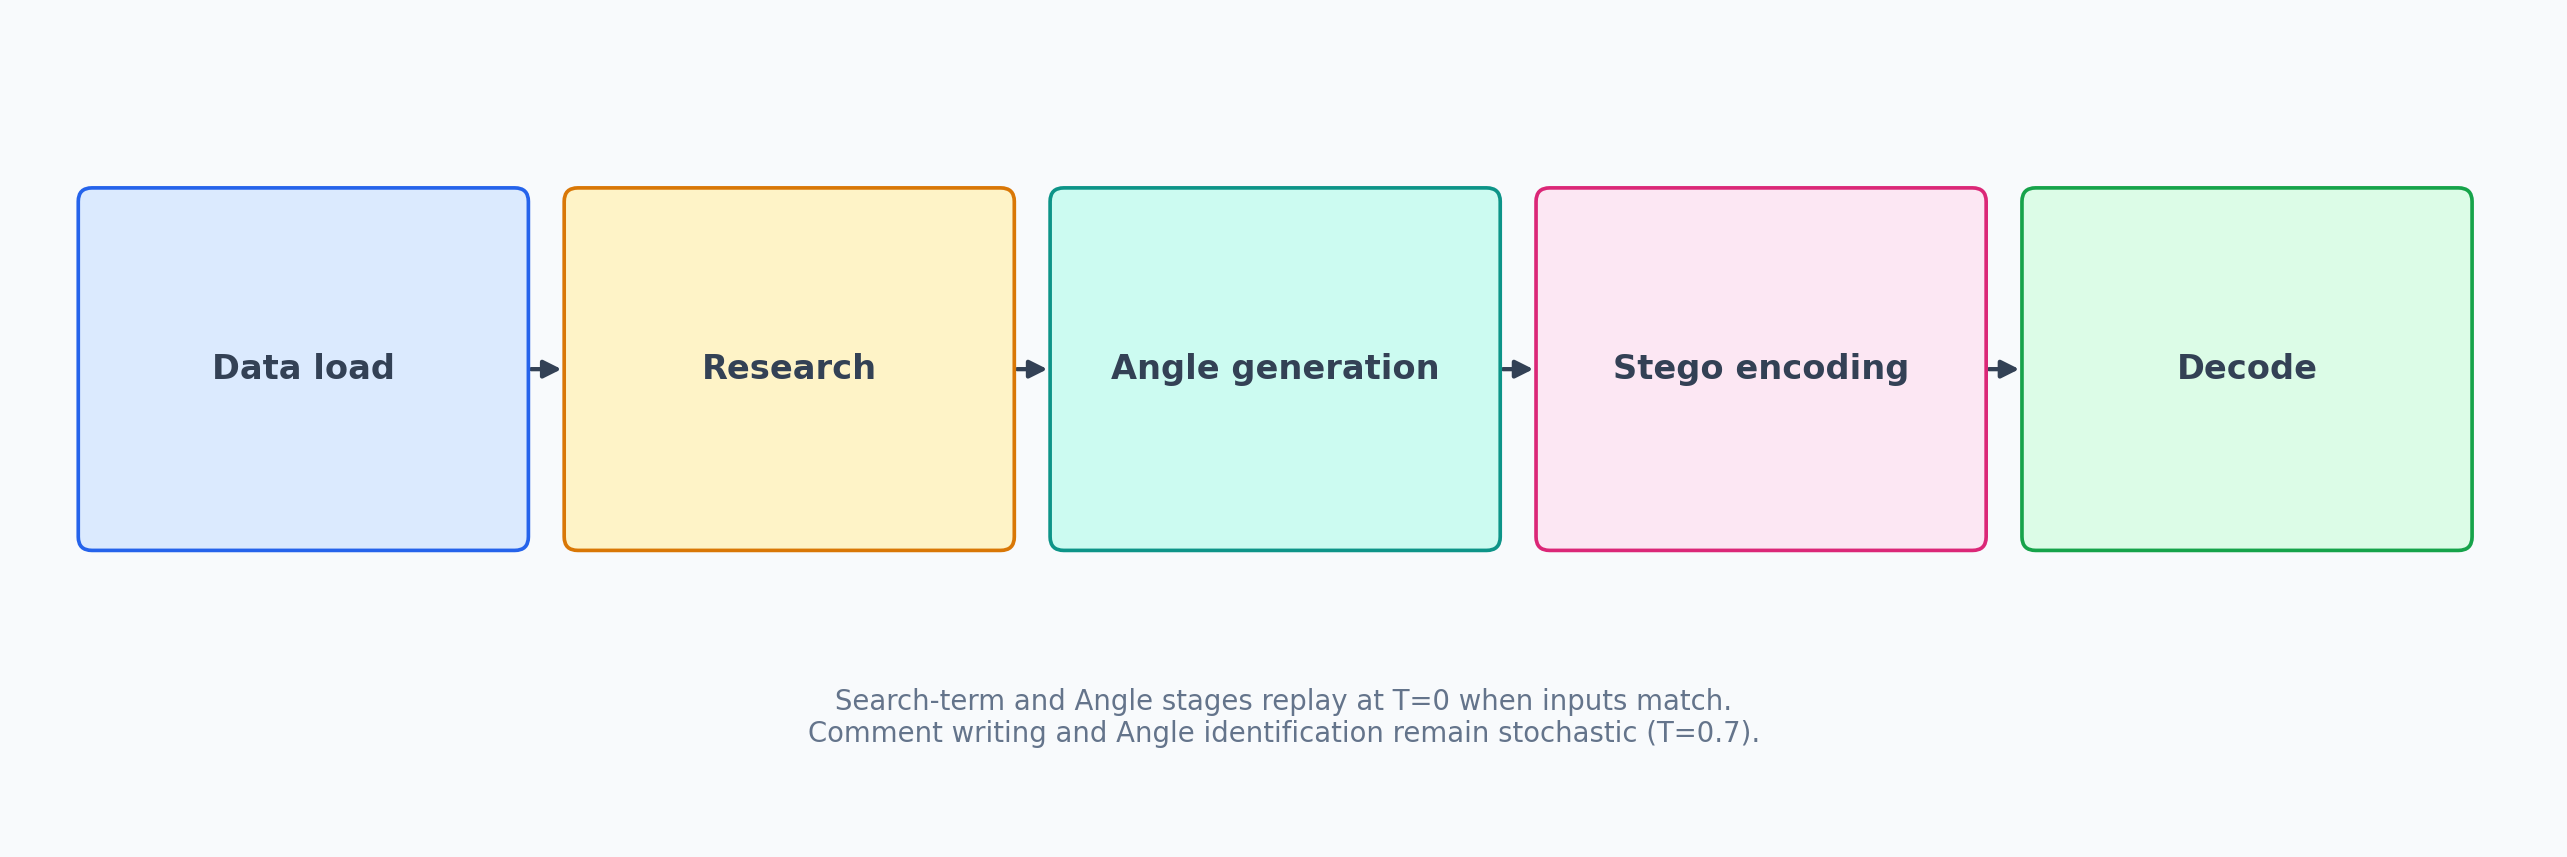
\includegraphics[width=\textwidth,height=0.55\textheight,keepaspectratio]{figures/implementation_pipelines}
	\Description{Block diagram of implementation pipeline stages and on-disk artifacts supporting replay and sender--receiver alignment.}
	\caption{Implementation stages and persisted artifacts. Search-term and Angle stages replay at temperature 0 when the inputs match; comment writing and Angle identification remain stochastic.}
	\label{fig:impl-pipelines}
\end{figure*}

\subsection{Model roles}
Exact model IDs are configuration.
The roles are not:
\begin{itemize}
    \item Search-term generation and Angle extraction run at \texttt{temperature=0} so both parties can rebuild the same lists from the same inputs.
    \item Comment writing runs at nonzero temperature (0.7 on balanced) so retries produce different wording for the same parent and Angle.
    \item Angle identification uses MiniLM cosine similarity, a default shortlist of 20 with lexical rerank, then the same stego temperature for an \texttt{idx: N} prompt. It is not a temperature-0 oracle.
\end{itemize}
